\documentclass[12pt]{article}
\usepackage[paper=a4paper,left=20mm,right=20mm,top=30mm,bottom =30mm]{geometry}
\usepackage[utf8]{inputenc}
\usepackage[T1]{fontenc}
\usepackage{stmaryrd}
\usepackage{setspace}
\usepackage{mathrsfs}
\usepackage[ngerman]{babel}
\usepackage{amssymb}
\usepackage{amsmath}
\usepackage{fancyhdr}
\usepackage[dvips,unicode,colorlinks,linkcolor=black]{hyperref} 
\usepackage{graphicx}
\usepackage{float}

\pagestyle{fancy}
\lfoot{}
\rfoot{Paul Kremser, Tobias Grussenmeyer}
\cfoot{\thepage}
\fancyhead[L]{FPI Versuch: Lange Halberwertszeiten}
\renewcommand{\headrulewidth}{0.6pt}
\renewcommand{\footrulewidth}{0.6pt}
\setlength{\headheight}{16pt}
\setlength{\parindent}{0pt}
% Für die Wahl der Schriftart
\newcommand{\changefont}[3]{
\fontfamily{#1} \fontseries{#2} \fontshape{#3} \selectfont}

\begin{document}
% keine Hurenkinder und Schusterjungen
\clubpenalty = 10000
\widowpenalty = 10000 
\displaywidowpenalty = 10000

\onehalfspacing
% Schriftart
\changefont{ptm}{m}{n} 

\begin{titlepage}
\author{Paul Kremser, Tobias Grussenmeyer}
\title{Versuch: Lange Halbwertszeiten}
\date{Versuchsdurchführung: 6. und 7. Oktober 2009} 
\maketitle
\thispagestyle{empty}
\end{titlepage}


\tableofcontents
\thispagestyle{empty}
\newpage
\pagenumbering{arabic}
\section{Überblick}
In diesem Versuch werden die Halbwertszeiten des $\alpha$-Strahlers $ ^{147}Sm$ und des $\beta$- Strahlers $^{40}K$ bestimmt. Da es sich um extrem langlebige Nuklide handelt $(T_{\frac{1}{2}} =1.06 \cdot 10^{11}$s  bzw.$1.28 \cdot 10^9$ Jahre) ist eine Beobachtung der Änderung der Impulsrate in Abhängigkeit von der Zeit nicht mehr möglich. Die Halbwertszeit $T_{\frac{1}{2}}$ lässt sich jedoch aus der spezifischen Aktivität $A_s$ bestimmen. Zur experimentellen Durchführung wird ein Methan-Durchflußzählrohr verwendet. Die radioaktiven Präparate (mit Aktivitäten < $200 Bq$) werden in ein direkt unter dem Zählrohr befindliches Probenrad eingebracht. Bei jeweils fest gewählter Hochspannung in den Plateaubereichen des Zählrohres werden die Aktivitäten der Präparate gemessen. Aus dem Zerfallsgesetz $A = ln(2) \frac{N}{T_{\frac{1}{2}}}$ kann bei bekannter Zahl der zerfallenden Atome N und nach einer Bestimmung der Aktivität A die Halbwertszeit $T_{\frac{1}{2}}$ berechnet werden. Zur Bestimmung der absoluten, d.h. durch Effekte wie Selbstabsorption und Rückstreuung nicht verfälschten, Aktivität aus den tatsächlich gemessenen Aktivitäten werden verschiedenen Methoden verwendet: Die Aktivität des $\alpha$-Strahlers Samarium wird
unter Ausnutzung der konstanten Reichweite der Strahlung und der bekannten Oberfläche des Präparats korrigiert. Beim $\beta$-Strahler Kalium wird die Massenabhängigkeit der beobachteten Aktivität ausgenutzt.


\section{Aufgabenstellung}
In diesem Versuch werden die Halbwertszeiten des $\alpha$-Strahlers $^{147}Sm$ und des $\beta$-Strahlers $^{40}K$ bestimmt. Da es sich dabei um sehr langlebige Nuklide handelt, ist eine direkte Bestimmung der Halbwertszeit aus der Beobachtung der Zeitabhängigkeit der Impulsrate nicht mehr möglich. Stattdessen werden die Halbwertszeiten aus der Aktivität der Präparate bestimmt. Bestimmung der Halbwertszeit von $^{147}Sm$ ($\alpha$-Zerfall)
\begin{enumerate}
 \item Bestimmung der Halbwertszeit von $^{147}Sm$ ($\alpha$-Zerfall)
\begin{itemize}
 \item Aufnahme der Zählrohrcharakteristik mit einem Natururan-Präparat
 \item Wahl des Arbeitspunktes auf dem $\alpha$-Plateau
 \item Messung des Nulleffekts
 \item Ermittlung der Aktivität des Samarium-Präparats (raumwinkelabhängige Messung)
\end{itemize}
\item Bestimmung der Halbwertszeit von $^{40}K$ ($\beta ^-$-Zerfall, EC)
\begin{itemize}
\item Aufnahme des $\beta$-Plateaus mit dem Kalium Präparat
\item Wahl des Arbeitspunktes auf dem $\beta$-Plateau
\item Messung des Nulleffekts
\item Ermittlung der spezifischen Aktivität des Kalium-Präparats (massenabhängige Messung)
\end{itemize}
\end{enumerate}

\section{Theoretische Grundlagen}
\subsection{Zerfallsgesetz und Aktivität}
Beim radioaktiven Zerfall ist die Wahrscheinlichkeit das ein Teilchen in einem Zeitintervall $dt$ zerfällt bestimmt durch die \textit{Zerfallskonstente} $\lambda$. Diese Wahrscheinlichkeit beträgt $\lambda dt$, bei $N$ Teilchen die zerfallen können zerfallen also im nächsten Zeitintervall $N\lambda dt$ Teilchen. Daraus ergibt sich das Zerfallsgesetz zu
\begin{align}
 N(t) = \int \limits_{0} \limits^{t} dN = \int \limits_{0} \limits^{t} - \lambda N dt = N_0 e^{-\lambda t}
\end{align}

wobei $N_0$ die zerfallsfähigen Teilchen zur Zeit $t=0$ angibt.\\
Die \textit{Halbwertszeit} $T_{\frac{1}{2}}$ eines Stoffes gibt an wie lange es dauert bis die Hälfte der Teilchen zerfallen sind. Es folgt also
\begin{align}
N(T_{\frac{1}{2}} = \frac{1}{2} N_0 = N_0 e^{ -\lambda T_{\frac{1}{2}}} \Rightarrow T_{\frac{1}{2}} = \frac{ln(2)}{\lambda}
\end{align}

Unter der \textit{Aktivität} $A$ versteht man die Anzahl der zerfallenden Teiclhen pro Zeit also 
\begin{align}
 \label{Aktivität} A = -\frac{dN}{dt} = \lambda N
\end{align}
Unsere Stoffe haben im Überblick beschrieben sehr Lange Halbwertszeiten, so dass man die Aktivität hier durchaus als konstant annehmen kann. Somit folgt für unsere Halbwertszeit:
\begin{align}
 \label{Halbzeit} T_{\frac{1}{2}} = \frac{N ln(2)}{A}
\end{align}

\subsection{Zerfallsarten}

Beim Radioaktiven Zerfall gibt es unterschiedliche Prozesse bei der verschiedene Zerfälle stattfinden. Dabei werden auch unterschiedliche Arten Radioaktiver Strahlung emittiert.

\begin{itemize}
 \item $\alpha$ Zerfall \\
Ein angeregte Atom geht unter aussendung eines Helium-Kerns in einen stabileren Zustand über. Alle $\alpha$-Teilchen eines bestimmten Übergangs weisen dieselbe Energie auf, da die beteiligten Niveaus diskret sind und nur ein Teilchen emittiert wird. Die Zerfallsgleichung für $^{147}Sm$ lautet:
\begin{align}
 \notag ^{148}_{62}Sm \longrightarrow ^{144}_{60}Nd + ^4_2He
\end{align}

\item $\beta^-$ Zerfall \\
Ein Neutron geht im Kern unter aussendung eines Elektrons und eines Antineutrinos in ein Proton über. Für den von uns verwendeten Beta Strahler $^{40}K$ lautet die Zerfallsgleichung:
\begin{align}
 \notag ^{40}_{19}K \longrightarrow ^{40}_{20}Ca + e^- + \overline{\nu_e}
\end{align}

\item $\beta^+$ Zerfall \\
Ein Proton geht im Kern unter aussendung eines Positrons und eines Neutrinos in ein Neutron über. Dieser Prozess kommt in der Natur nur sehr selten vor. Das Positron kann hier in Gegenwartvon Materie nicht existieren, es vereint sich mit einem Elektron zu einem Positronium-Atom, welches innerhalb kürzester Zeit unter aussendung zweier Photonen zerfällt. Also lautet die Zerfallsgleichung für unseren Strahler:
\begin{align}
 \notag ^{40}_{19}K \longrightarrow ^{40}_{18}Ar + e^+ + \nu_e
\end{align}

\item Elektroneneinfang (\dq EC = electron capture\dq ~oder auch  \dq$\epsilon$ Zerfall\dq) \\
Ein Elektron aus der Hülle wird vom Kern eingefangen, wodurch ein Proton unter aussendung eines Neutrinos zu einem Neutron umgewandelt wird. Die Zerfallsgleichung für $^{40}K$ lautet:
\begin{align}
 \notag ^{40}_{19}K + e^- \longrightarrow ^{40}_{18}Ar + \nu_e
\end{align}
\end{itemize}

\subsection{Reichweite}

Beim Durchgang von $\alpha$-Teilchen durch Materie wechselwirken diese mit den Atomhüllen, also den Elektronen. Da die Heliumkerne viel schwerer sind als Elektronen, werden $\alpha$-Strahlen beim Durchgang durch Materie nicht abgelenkt. Desweiteren wird bei einem Ionisationsprozess nur relativ wenig Energie abgegeben, es sind also sehr viele solche Ionisationen notwendig um ein Teilchen zu bremsen. Daher haben $\alpha$-Teilchen gleicher Energie auch annähernd die gleiche Reichweite, wesshalb man aus der Reichweite hier auf die Energie schliessen kann. 

Für die maximal Reichweite existiert eine Näherungsformel von Bragg und Cleeman: 
\begin{align}
 \label{cleeman} R \rho=c\sqrt{m_A}
\end{align}
wobei $\rho$ die Dichte, $m_A$ das effektive Atomgewicht und $c$ eine Proportionalitätskonstante ist.
\\ \\
Für $\beta$ Strahlung gilt dies nicht mehr, da Elektronen viel leichter sind verlieren sie durch Ionisation bzw Anregen eies anderen Elektrons relativ viel Energie, und werden zusätzlich stark gestreut. Daher kann man die Reichweite nicht genau angeben, sondern nur einen Maximalwert (der Elektronen die doch geradlinig, ohne Energieverlust durch die Materie kamen).


\subsection{Gasionisationsdetektoren}

Bei dieser Messaperatur wird die Ionisierende Wirkung radioaktiver Strahlung ausgenutzt um diese zu messen. Sie besteht aus einer gasgefüllten Kammer deren Wand als Kathode genutzt wird und einem Zähldraht, der Anode. Die Gasionen ereugen einen Spannungsimpuls der zur detektion genutzt wird. Die Impulsgrösse (die Anzahl der Elektronen die die Anode ereichen) ist dabei abhängig von der angelegten Spannung. Hier gibt es für verschiedene Anwendungen verschieden Arbeitsbereiche, in unserem Versuch verwenden wir ein Propotionalitätszählrohr, dh die Impulsgrösse ist verstärkt, aber proportional zur Anfangsionisation. Eine andere Anwendung, welche im sogenanten Auslösebereich arbeitet ist das Geiger-Müller-Zählrohr. Hier findet eine lawinenartige Entladung statt, so das jede Ionisation einen sehr grossen Impuls auslöst. Da sich das Gas durch Ionisation auch verbraucht, verwenden wir win Durchflusszählrohr, dh das Gas wird ständig erneuert.

\subsection{Berechnung der Halbwertszeit von Samarium}
Da die $\alpha$-Teilchen in Samarium eine maximale Reichweite R haben, können nur die austreten, deren Weglänge r in Samarium kürzer als R ist. Der Zusammenhang zwischen Raumwinkel $\theta_{max}(z)$ den das Teilchen noch haben darf um die Probe zu verlassen und der Tiefe z des zerfallenen Teilchens ist dabei aus Abbildung \ref{winkel} ersichtlich.
Da $\theta = arccos(\frac{z}{r})$ wird dies maximal für $r=R$ also:
\begin{align}
 \theta_{max}(z) = arccos\left( \frac{z}{R} \right)
\end{align}

\begin{figure}[H]  
\centering
\label{winkel} \includegraphics[width=0.5\linewidth]{pictures/winkel.ps}
\caption{Austrittswinkel}
\end{figure}

Also gilt für den maximalen Raumwinkel in abhängigkeit der Tiefe:
\begin{align}
 \omega(z)= \int \limits^{2\pi} \limits_{0} d\phi = \int \limits^{\theta_{max}(z)} \limits_{0} sin(\theta)d\theta = 2\pi \left( 1 - \frac{z}{R} \right) 
\end{align}

Für die Zählrate n gilt:
\begin{align}
 n = \frac{a_V F}{4 \pi} \int \limits_0 \limits^R \omega (z) dz = \frac{A_V F R }{4}
\end{align}
wobei $A_V$ die Aktivität pro Volumen und $F$ die Oberfläche der Probe ist. Berücksichtigt man $A=A_V V = A_V F h$ wobei $h$ die höhe der Probe ist so folgt für die Halbwertszeit $T_{\frac{1}{2}}$:
\begin{align}
 T_{\frac{1}{2}} = \frac{N ln(2)}{A} = \frac{N ln(2)}{A_V F h} = \frac{R N ln(2)}{4 n h}
\end{align}

Die maximal Reichweite ist uns hierbei nicht bekannt, wir können aber die Beziehung (Gleichung \ref{cleeman}) von Bragg und Cleeman ausnutzen. Die Proportionalitätskonstante lässt sich durch die bekannten Werte für Luft eliminieren, und es folgt für Samariumoxyd:
\begin{align}
 R_{Sm_2O_3} \rho_{Sm_2O_3} = R_{Luft} \rho_{Luft} \sqrt{\frac{m_{A,Sm_2O_3}}{m_{A,Luft}}}
\end{align}
wobei sich $m_A$ folgendermassen berechnet:
\begin{align}
 \sqrt{m_A}=\sum \limits_i p_i \sqrt{m_{A_i}}
\end{align}
$m_{A_i}$ bezeichnet das Atomgewicht eines Elements und $p_i$ der relative Anteil dieser Atome an der Substanz

Als letztes fehlt uns noch die Anzahl $N$ der zerfallsfähigen $^{147}Sm$ Kerne. Die Anzahl $N_{Sm_2O_3}$ der Samariumoxydmoleküle erhält man durch:

\begin{align}
 N_{Sm_2O_3} = \frac{m N_A}{m_{r,Sm_2O_3}}
\end{align}

wobei m die Masse des Präparats, $m_{r,Sm_2O_3}$ die relative Molekülmasse von Samariumoxyd in $g/maol$ und $N_A$ die Avogadrozahl ist.
Berücksichtigt man die relative Häufigkeit $h_{rel} = 0.1487$ von $^{147}Sm$ in Samarium und $m = \rho V = \rho F h$ erhält man für die gesuchte Anzahl $N$:
\begin{align}
 N=2N_{Sm_2O_3} h_{rel}= 2 \frac{m N_A}{m_{r,Sm_2O_3}} h_{rel}=2 \frac{\rho F h N_A}{m_{r,Sm_2O_3}}h_{rel}
\end{align}

und schliesslich erhält man also für die Halbwertszeit von $^{147}Sm$:
\begin{align}
 T_{\frac{1}{2}} = \frac{R N ln(2)}{4 n h} = \frac{R \rho  N_A h_{rel} ~ ln (2)}{2n m_{r,sm_2O_3}} F
\end{align}

\label{kalium}\subsection{Berechnung der Halbwertszeit von Kalium}

Beim Kalium kommt es neben dem von uns messbaren $\beta^-$ Zerfall noch
 zu $\beta^+$ Zerfall und Elektroneneinfang, beide Effekte werden bei unserer
 Messung nicht berücksichtigt. Desweiteren kommt es zu Selbstabsorbtion und Rückstreuung 
am Probenbehälter. Das Verhältniss der Wahrscheinlichkeiten von $\beta^-$ Zerfall zu der
 von $\beta^+$ und Elektroneneinfang ist bekannt und beträgt:
\begin{align}
 \frac{P(\beta^-)}{P(\beta^+ \bigcup EC)} = \frac{100}{13}
\end{align}

Also gilt für die Zerfallskonstante $\lambda_K$ von Kalium:
\begin{align}
 \lambda_K=\lambda_{\beta^-} + \lambda_{\beta^+,EC}=1,13\lambda_{\beta^-}
\end{align}

Es wird nur die Anzahl der $\beta^-$ Zerfälle gemässen, also die Aktivität $A_{\beta^-}$. Mit Gleichungen \ref{Aktivität} und \ref{Halbzeit} folgt also für die Halbwertszeit:
\begin{align}
\label{zeit} T_{\frac{1}{2}} = \frac{ln(2)}{\lambda_K} = \frac{ln(2)}{1,13 \lambda_{\beta^-}} = \frac{1}{1,13} \frac{ln(2) N}{A_{\beta^-}} = \frac{T_{\frac{1}{2}, \beta^-}}{1,13}
\end{align}

Selbstabsoption bedeutet das die emitierten Elektronen im innern der Probe reabsorbiert werden bevor sie diese veralssen können. Dabei lässt sich über die Zählrate $n$ sagen:
\begin{align}
 dn=\rho F D e^{-\mu x} dx
\end{align}
dabei ist $\rho$ die Dichte, $F$ die Oberfläche der Probe, D die spezifische Aktivität (pro Masse) und $\mu$ der Absorptionskoeffizient. Integriert bis zur Höhe $h$ der Probe, die wir über die Masse ausdrücken können mittels $h = \frac{m}{F \rho}$ ergibt sich:
\begin{align}
  \label{zählrate} n(m) = \int \limits_{0} \limits^{\frac{m}{F \rho}} \rho F D e^{-\mu x} dx = \frac{\rho F D}{\mu} \left( 1- e^{-\frac{\mu}{F \rho} m} \right) = a \left( 1 - e^{-bm} \right)
\end{align}

Nun kann man die Masse $m$ bei der Messung variieren und über eienen Fit an obige Funktion die Parameter $a$ und $b$ bestimmen. Nun muss noch die Rückstreuung am Aluminiumbehälter berücksichtigt werden. Dazu nutzt man eine folgende Beziehung die für die Tangente an $n(m)$ im Punkt $M=0$ gelten muss:
\begin{align}
 \left. \frac{dn}{dm}  \right|_{m=0} = D f_B \frac{\omega}{4\pi}
\end{align}

wobei für uns der Rückstreufaktor $f_B$ für Aluminium $1,29$ beträgt und der Raumwinkel $\Omega=2\pi$ ist. Leitet man Gleichung \ref{Zählrate} ab und nutzt diese Beziehung so folgt:
\begin{align}
  \left. \frac{dn}{dm}  \right|_{m=0} = ab =  D f_B \frac{\Omega}{4\pi}
\end{align}

also folgt für die Aktivität
\begin{align}
 A_{\beta^-}=m D=\frac{2ab}{f_B}m
\end{align}

Zuletzt fehlt noch die Anzahl $N$ der ${40}^K$ Kerne in unserer Probe. Diese haben in natürlichem Kalium eine relative Häufigkeit von $h_{rel}=0,0118\%$§. Mit der relativen molekülmasse $m_{KCl}$ von Kaliumoxyd in $g/maol$ und der Avogadrozahl $N_A$ ergibt sich die gesuchte Anzahl zu:
\begin{align}
 N=\frac{m N_A}{m_{KCl}} h_{rel}
\end{align}

Nun kennen wir alle Grössen und Korekturen zur berechnung der Halbwertszeit. Sie beträgt nach Gleichung \ref{zeit}:
\begin{align}
 T_{\frac{1}{2}} = \frac{N_A h_{rel} ~ ln(2)}{1,13 D m_{KCl}}
\end{align}
\newpage

\section{Versuchsaufbau}

\begin{figure}[H]  
\centering
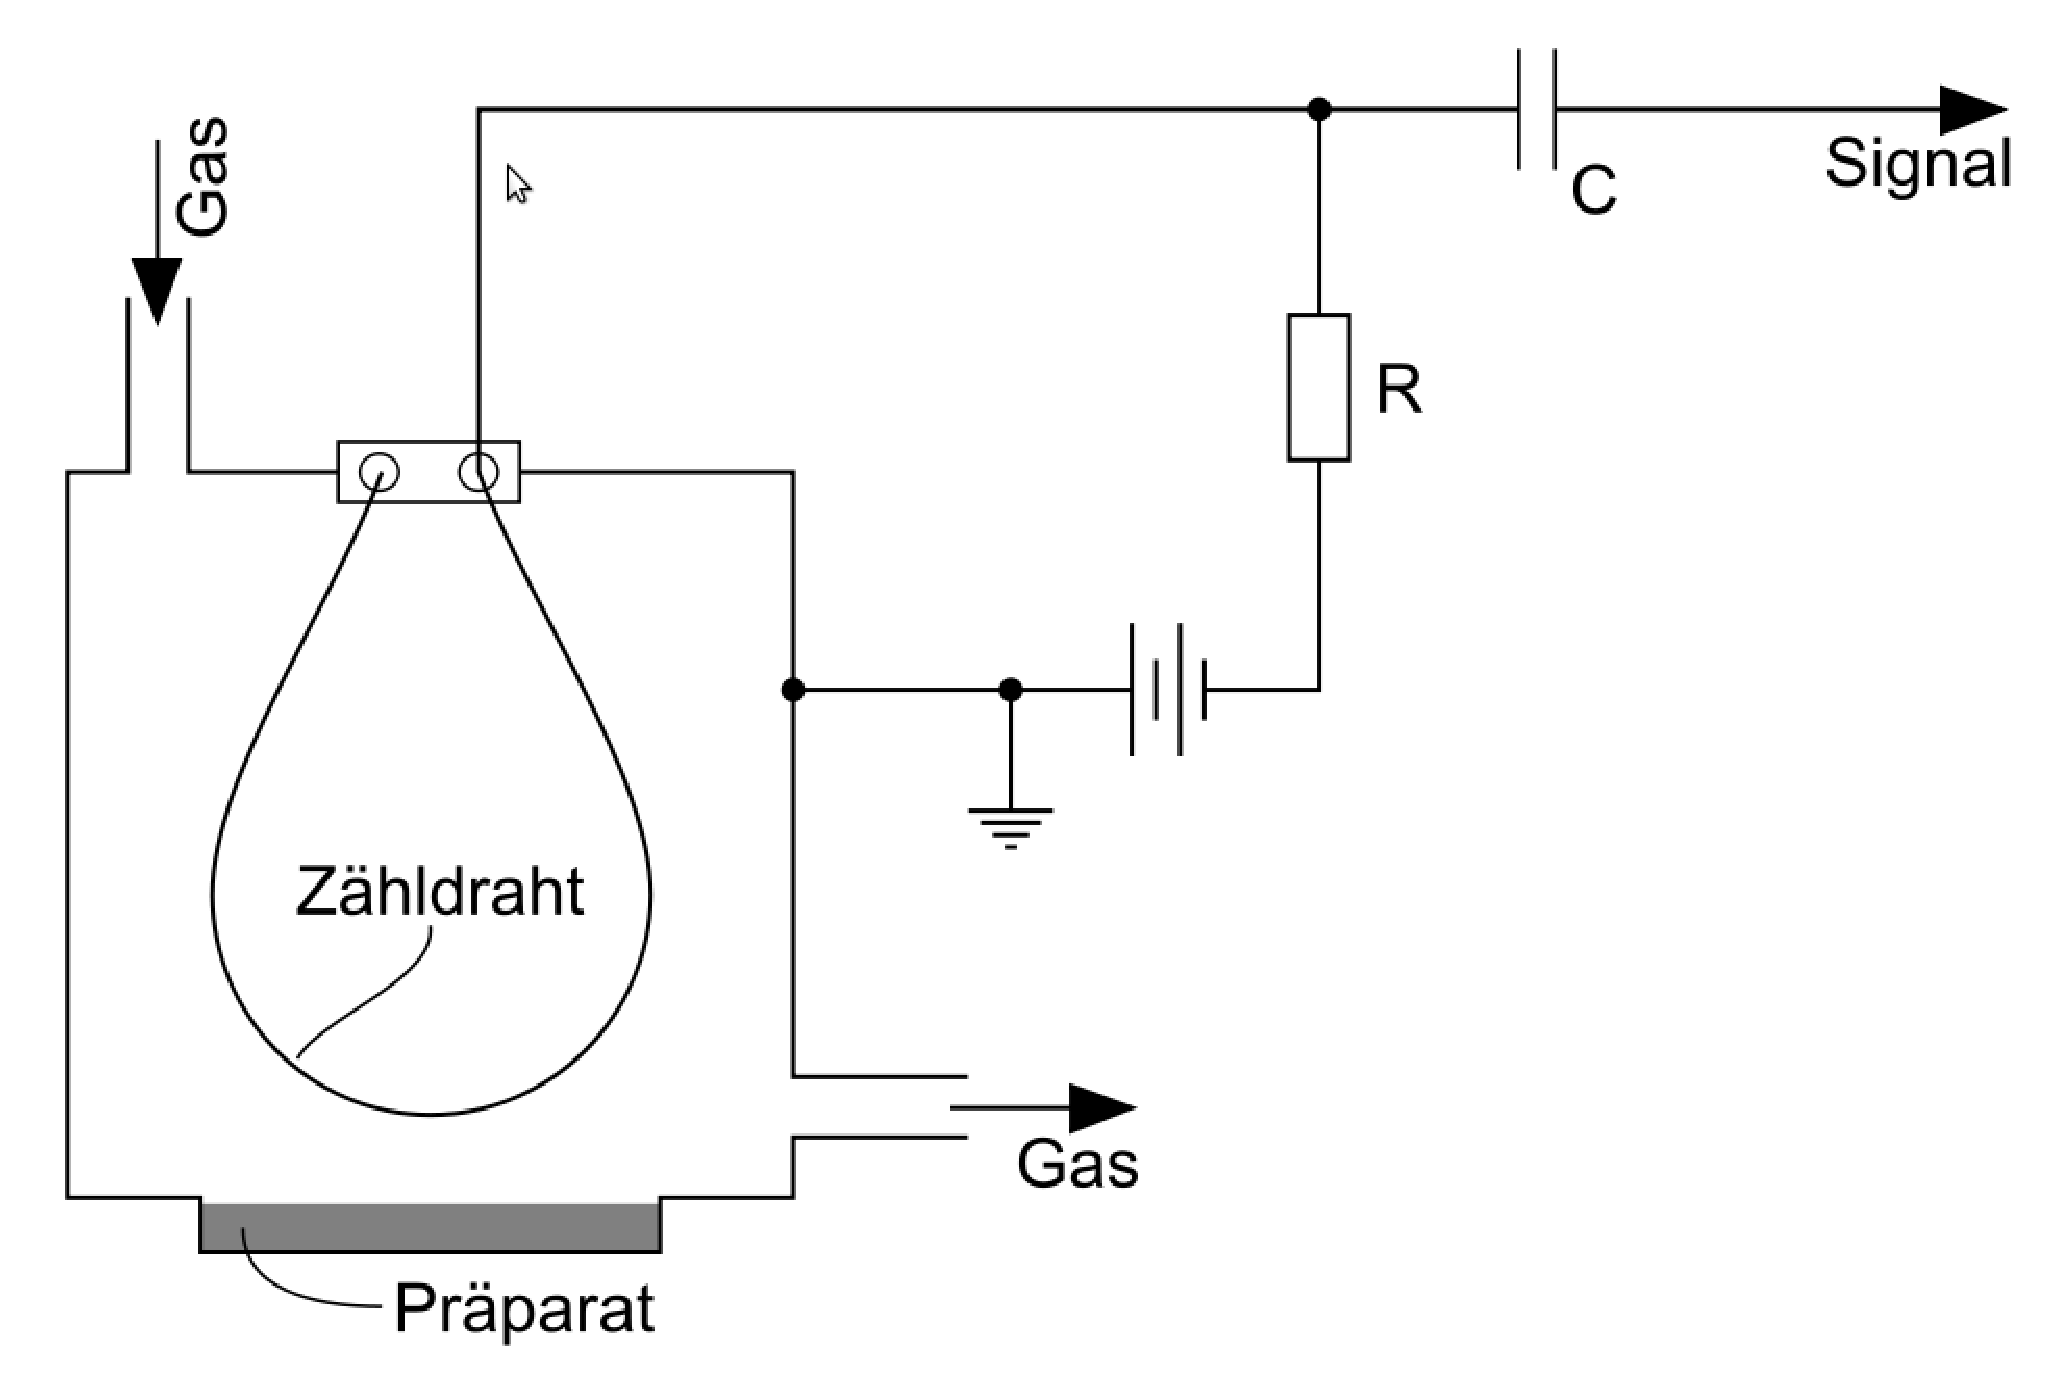
\includegraphics[width=0.9\linewidth]{pictures/aufbau.eps}
\caption{Durchflusszählrohr}
\label{aufbau}
\end{figure}

Für die Messung steht ein Methandurchflusszählrohr (Abb. \ref{aufbau}) zur Verfügung.
Dieses wird im Proportionalbereich betrieben. Zwischen Zähldraht und Gehäuse liegt eine Hochspannung von bis zu 4$kV$ an.
Um das zu vermessende Präparat in die Zählkammer zu bekommen wird dieses auf einen Drehteller gesetzt und dieser in die Kammer gedreht.
Das entstehende Signal wird über einen Kondensator ausgekoppelt und mittels Verstärker auf einen Eingang am PC getriggert. Außerdem kann
es auf dem Oszilloskop beobachtet werden.

\section{Durchführung}
Zu Beginn arbeiteten wir mit einer Uranprobe um die Zählrohrcharakteristik aufzunehmen und überhaupt die Aperatur kennen zu lernen.

Anfangs versuchten wir Einstellungen der Elektronik zu finden bei denen die Zählrate maximal ist, jedoch war darauf zu achten dass keine Teilchen doppelt
gezählt werden. Wir entschieden uns für folgende Einstellungen:
\begin{itemize}
 \item Verstärker: Gain 7,20; Coarse Gain 20; Shaping Time 1$\mu s$
 \item Timing SCA: low level 3,0; high level 10,0; delay 1,0
 \item Gate: delay 1,0 $\cdot$ 1,1$\mu s$
\end{itemize}

Mit diesen Einstellungen nahmen wir die Uran-messung vor.
Anschließend wurde ebenfalls mit diesen Einstellungen die Samariummessung durchgeführt.

Für die Messung mit Kalium verwendeten wir andere Einstellungen aber hierzu später.

\section{Auswertung}
\subsection{Zählrohrcharakteristik mit Uran}


Zu Begin machten wir eine Messung mit einem Uranpräparat um die Charakteristik des Zählrohrs kennen zu lernen.
Hierzu gingen wir in 100$V$ Schritten von 1000$V$ bis 4000$V$ mit einer jeweiligen Messdauer von 50$s$.
Außerdem machten wir mit den selben Einstellungen eine Untergrundmessung von von 1600 bis 4000$V$ mit jeweils 100$s$
Messdauer und verwendeten diese um die Zählrohrcharakteristik zu korrigieren.

Der Fehler auf die Zählrate berechnet sich dann wie folgt:
\begin{align}
 s_n = \frac{s_N}{t} = \frac{\sqrt{N}}{t} = \frac{\sqrt{n~t}}{t} = \sqrt{\frac{n}{t}}
\end{align}

Mit Gesamtanzahl der Counts $N$, Fehler auf diese $s_N$, Zählrate $n$ und jeweilige Messdauer $t$. Wobei wir den Fehler auf die Messdauer
vernachlässigen.


\begin{figure}[H]  
\centering
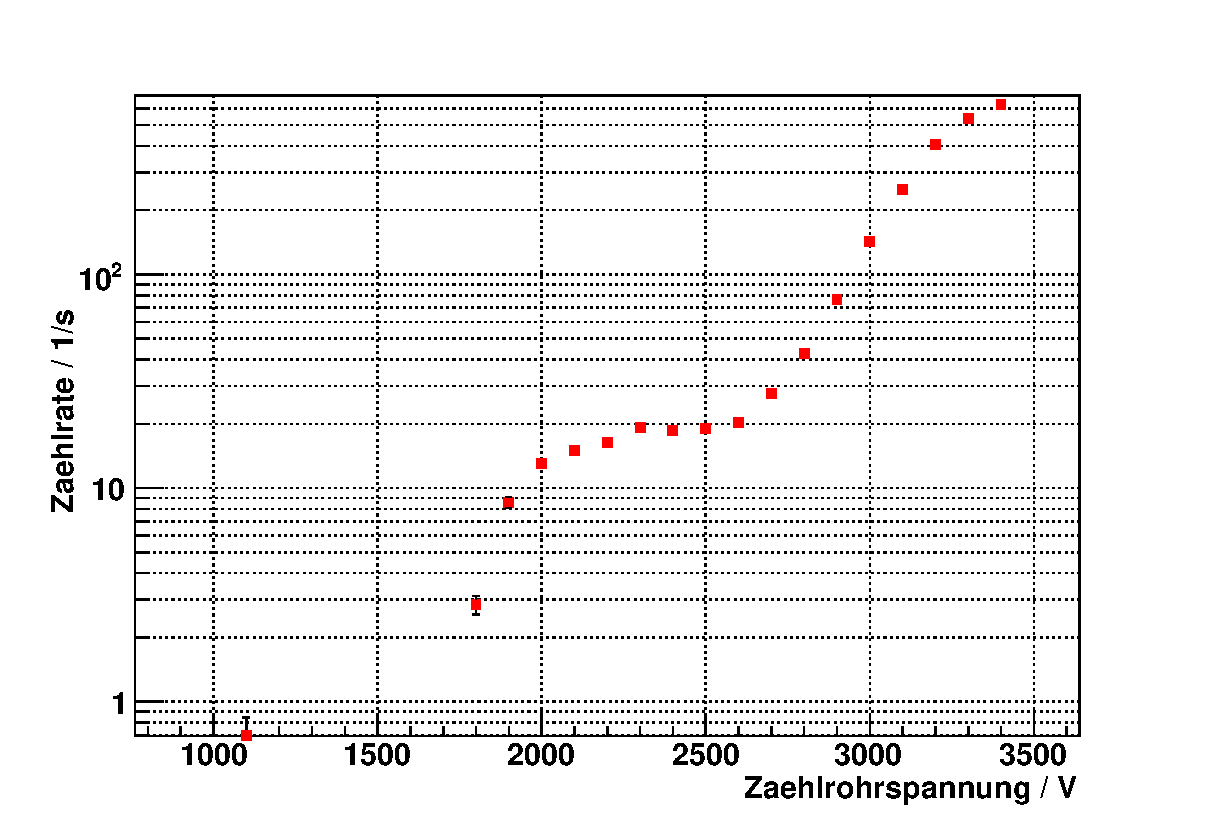
\includegraphics[width=0.9\linewidth]{pictures/char_uran.eps}
\caption{Zählrohrcharakteristik mit Uran}
\end{figure}


\subsection{Halbwertszeit von Samarium}
Zuerst nahmen wir das $\alpha$-Plateau auf. Hierfür orientierten wir uns an der mit Uran aufgenommenen Charakteristik (1800-3400$V$).
Diese Messung geschah mit den selben Einstellungen wie die mit Uran und kann daher mit der selben Untergrundmessung korrigiert werden.

\begin{figure}[H]  
\centering
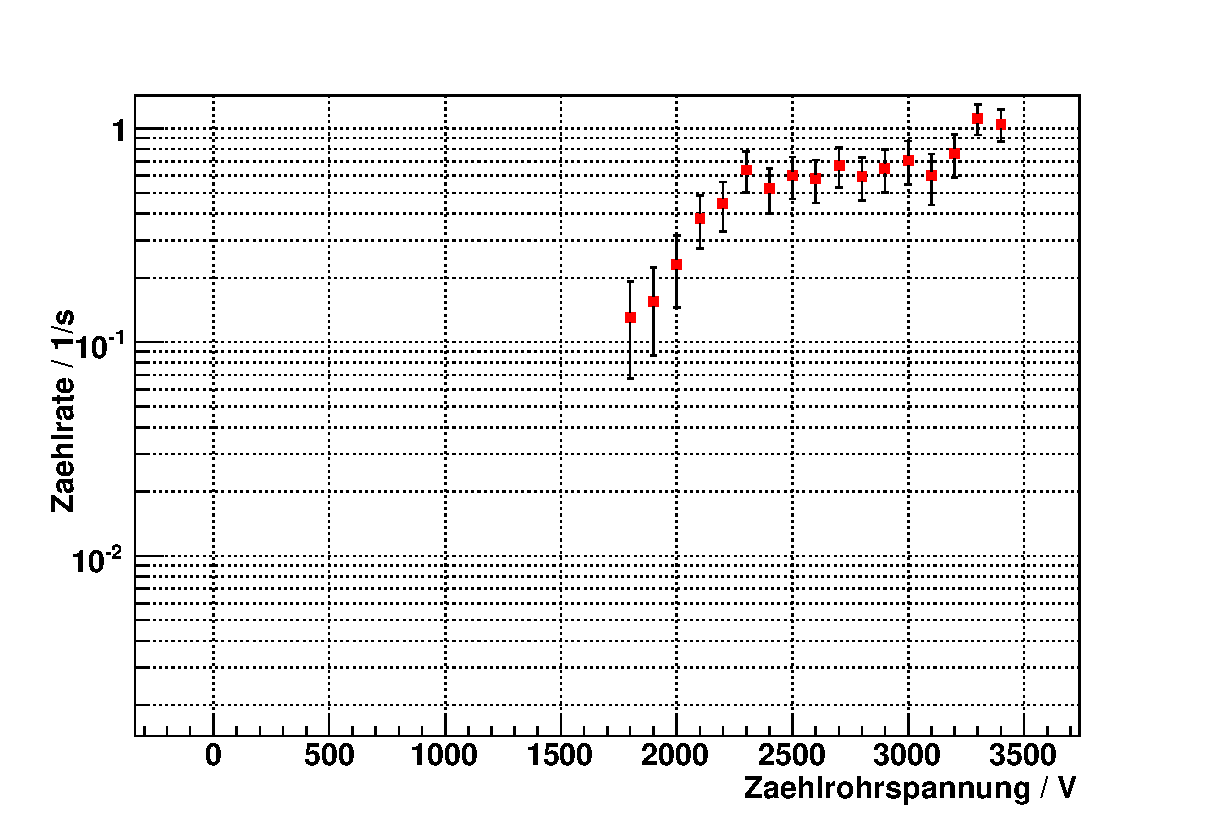
\includegraphics[width=0.9\linewidth]{pictures/char_sam.eps}
\caption{Zählrohrcharakteristik mit Samarium}
\end{figure}

Aus der Messung bestimmten wir demn Arbeitspunkt bei 2600$V$ und konnten mit der dort gemessenen Rate die benötigte Messzeit um den Messfehler unter
2\% zu bekommen berechnen (4300$s$). Ebenso konnten wir die Messzeit für die Untergrundmessung berechnen um einen Beitrag zum Fehler auf die Rate
von $1/3$ zu erhalten (3000$s$).

Die tatsächliche Rate $n$ setzt sich dann aus gemessener Rate $n^*$ und Untergrund $u$ zusammen: $n = n^* - u$. Wenn man auch hier wieder den Fehler auf
die Zeit vernachlässigt, erhält man für den Fehler:
\begin{align}
 s_n = \sqrt{s_{n^*}^2 + s_u^2} = \sqrt{\frac{n*}{t} + \frac{u}{t}} = 0,01 s^{-1}
\end{align}

Um den durchmesser der Probe zu bestimmen maßen wir diesen abwechselnd mit einer Schiebelehre und erhielten dabei zweimal 2,905 und achtmal 2,900.
Daraus ergibt sich ein Durchmesser von $d = (2,901~ \pm~ 0,0016)cm$ wenn man 0,005$cm$ als Ablesefehler annimmt. Was wiederum eine Fläche von
$F = \frac{\pi}{4}~d^2 = 6,606 cm^2$ mit einem Fehler von
\begin{align}
 s_F = \sqrt{\left(\frac{\partial F}{\partial d}\right)^2~s_d^2} = \frac{\pi}{2}~d~s_d = 0,007 cm^2
\end{align}
ergibt.

Mit Rate und Fläche lässt sich nun die Halbwertszeit bestimmen:
\begin{align}
T_{\frac{1}{2}} = \frac{R~\rho~ln 2 ~ N_A ~ h_{rel} ~ F}{2~m_{r,Sm_2O_3}~~n}
\end{align}

mit dem Fehler:
\begin{align}
 s_{t_{\frac{1}{2}}} = \sqrt{\left(\frac{s_F}{F}\right)^2 + \left(\frac{s_n}{n}\right)^2}~\cdot~t_{\frac{1}{2}}
\end{align}

Als Ergebins für die Halbwertszeit von $^{147}Sm$ erhielten wir:
\begin{align*}
T_{\frac{1}{2}} = (2,1518~\pm~0,0643)~\cdot~10^11~a
\end{align*}

Für die Berechnungen der Werte siehe Abschnitt %\ref{samarium}

\subsection{Zählrohrcharakteristik mit Kalium}
Da wir für sie Halbwertszeit von Samarium einen Wert erhielten der ungefähr das doppelte des Literaturwertes ist, entschieden wir uns die Einstellungen der Elektronik noch einmal zu verändern. Wir gingen davon aus, dass wir nicht alle Counts gezählt hatten und mussten daher die untere Schrankte des Timing SCA tiefer stellen. Außerdem veränderten wir die Shaping time. Wir arbeiteten also nun mit folgenden Werten:

\begin{itemize}
 \item Verstärker: Gain 14,35; Coarse Gain 20; Shaping Time 3$\mu s$
 \item Timing SCA: low level 0,3; high level 10,0; delay 1,0
 \item Gate: delay 1,0 $\cdot$ 1,1$\mu s$
\end{itemize}

Zu Begin nahmen wir die Charakteristik des $\beta$-Plateaus mit Kaliumchlorid auf. Hierfür fuhren wir von 2600 bis 4000$V$ in 100$V$ Schritten mit einer jeweiligen
Messdauer von jeweils 100$s$.
Da wir die Einstellungen verändert hatten mussten wir auch eine erneute Untergrundmessung durchführen. Wir nahmen die gleichen Spannungs und Zeiteinstellungen wie für die Messung.

\begin{figure}[H]  
\centering
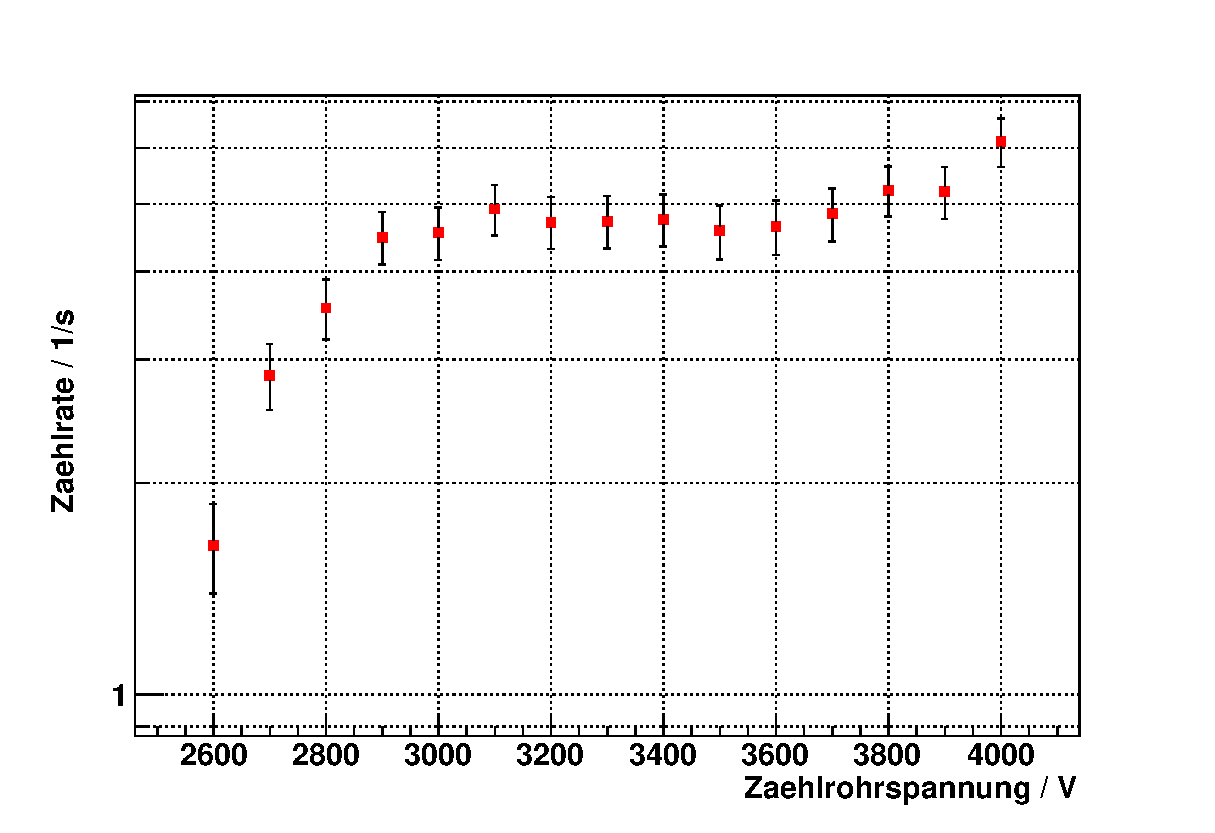
\includegraphics[width=0.9\linewidth]{pictures/char_kalium.eps}
\caption{Zählrohrcharakteristik mit Kalium}
\end{figure}

Nach Betrachtung der Grafik entschieden wir uns für einen Arbeitspunkt von 3400$V$.

\subsection{Bestimmumg der Halbwertszeit von Kalium}
Wir füllten ein Schälchen bis zum Rand mit Kaliumchlorid. Aus der gefüllten Schälchenmasse und der des leeren Schälchens berechneten wir die Massenschrittweite um äquidistante Punkte auf der x-Achse zu bekommen zu 0,1$g$ für 10 Messungen.

Wir begannen also mit der Messung mit vollständig gefülltem Schälchen und entfernten nach jeder Messung 0,1$g$ $KCl$. Die jeweilige Messdauer berechneten wir wieder aus Überlegungen zur Fehlergröße zu 460$s$. Am Schluss führten wir noch eine Untergrundmessung mit 865$s$ durch. Die Untergrundmessung wurde von den jeweiligen Messungen abgezogen.

\begin{figure}[H]  
\centering
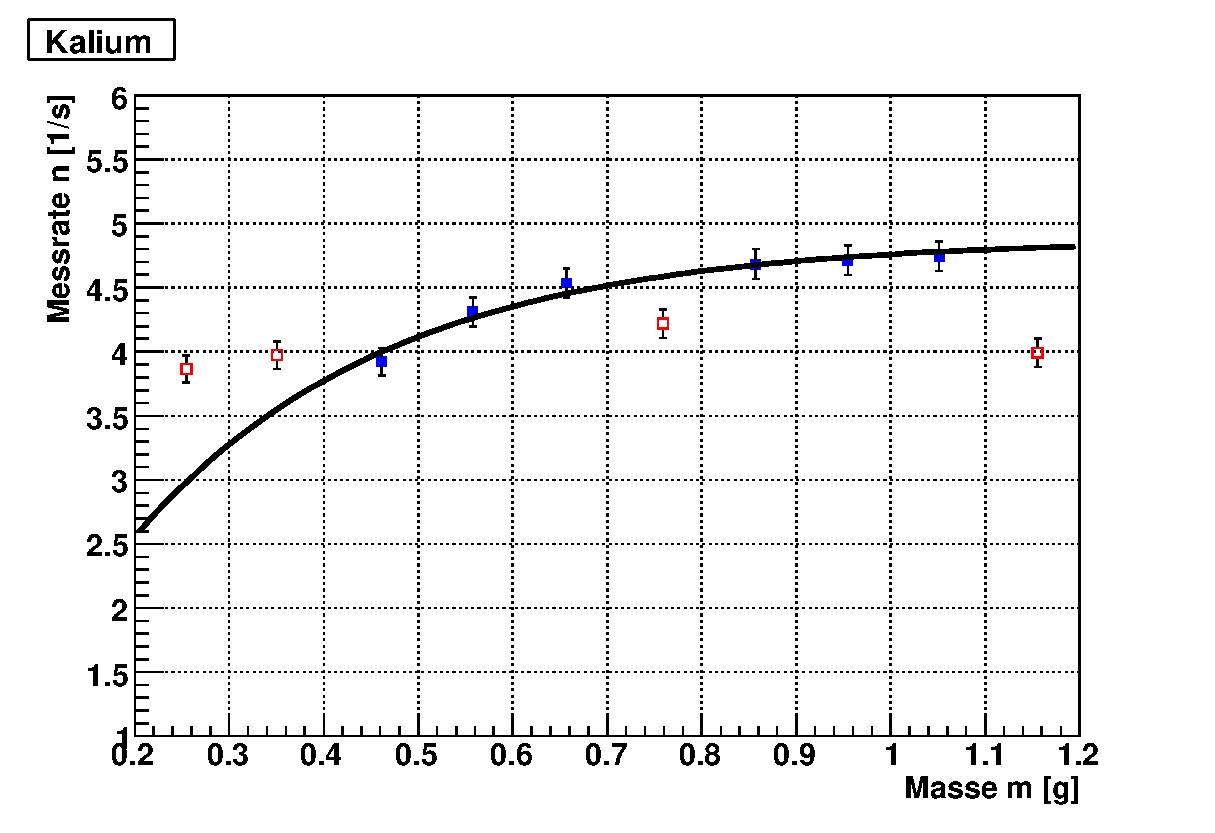
\includegraphics[width=0.9\linewidth]{pictures/kalium.eps}
\caption{Massenabhängigkeit mit Kalium}
\end{figure}

Um die Kurve an die Messung anpassen zu können mussten wir einige Messpunkte verwerfen (hier rot gekennzeichnet).
Mit den Parametern aus dem Fit ($a = 4~8789~\pm~0,1050$ und $b = 3,7128~\pm~0,3566$) lässt sich die spezifische Aktivität des $\beta$-Zerfalls bestimmen zu:
\begin{align*}
 D = 28,0842~\pm~2,7640
\end{align*}
und damit die Halbwertszeit zu:
\begin{align*}
T_{\frac{1}{2}} = (0,6602~\pm~0,0650)~\cdot~10^9~a
\end{align*}
Für die Berechnungen der Werte siehe Abschnitt 3.6
\newpage
\section{Zusammenfassung}
Unsere Messungen ergaben für
\begin{itemize}
 \item \textbf{Samariumoxid} eine Halbwertszeit von: $T_{\frac{1}{2}} = (2,1518~\pm~0,0643)~\cdot~10^{11}~a$
 \item \textbf{ Kaliumchlorid }eine Halbwertszeit von: $T_{\frac{1}{2}} = (0,6602~\pm~0,0650)~\cdot~10^9~a$
\end{itemize}
Wenn man die von uns erhaltenen Werte mit den Literaturwerten vergleicht:
\begin{align}
 \notag \textnormal{Samarium Halbwertszeit: }T_{\frac{1}{2}, Lit}^{Sm} &= 1,06~\cdot~10^{11}~a\\
 \notag \textnormal{Kalium Halbwertszeit: }T_{\frac{1}{2}, Lit}^K &= 1,28~\cdot~10^{9}~a
\end{align}
so stellt man fest, dass wir mit der ersten Einstellung der Elektronik wohl wie vermutet nicht alle Zerfälle registriert haben. Bei der folgenden Änderung der Einstellungen haben wir es dann aber wohl wieder etwas übertrieben, scheinbar haben sich hier einige Zerfälle ereignet die doppelt gezählt wurden.
Das doppeltzählen einzelner Zerfälle ist ein Vorgang der wohl auch schon von anderen Studenten beobachtet wurde. Verursacht wird er durch das Überschwingen des Verstärkers welches, wenn stark genug, auch als Zerfall gezählt wird. Um dies zu vermeiden wurde am Versuchsaufbau der Gate Generator hinzugefügt, er soll den Pegel des ersten Ausschlags so lange oben halten, dass der zweite verdeckt wird. Als wir die Einstellungen vornahmen beobachteten wir die verschiedenen Signale auf dem Oszilloskop und konnten dort keine Doppelausschläge sehen. Und das obwol wir eine Speichereinstellung gewählt hatten mit der man bei geringer Rate jeden Zerfall beobachten konnte. Wir gingen also nicht davon aus dass Doppelzählungen vorkommen würden.

Wenn man die von uns gemessenen Raten durch 1,6 teilt so kommt man direkt auf den Literaturwert. Scheinbar haben wir also in 37,5\% der gemessenen Zerfälle diese doppelt gemessen. 
Dies erscheint allerdigs sehr hoch dafür, dass wir nie einen Doppelausschlag auf dem Oszilloskop beobachten konnten. Möglicherweise liegen noch andere systematische Fehler vor.


\end{document}
